\chapter{Grid geometry}

\section{Horizontal grid}
The horizontal ICON grid consists of a set of spherical triangles that seamlessly span the entire sphere. The grid is constructed from an icosahedron (see Figure 
\ref{fig_ico_a}) which is projected onto a sphere. The spherical icosahedron (Figure \ref{fig_ico_b}) consists of $20$ equilateral spherical triangles. The edges of each triangle 
are bisected into equal halves or more generally into $n$ equal sections. Connecting the new edge points by great circle arcs yields $4$ or more generally $n^2$ spherical triangles 
within the original triangle (Figure \ref{fig_bisect}, \ref{fig_nsect}). 

\begin{figure}[h]
  \begin{minipage}[b]{0.4\textwidth}
    \centering
    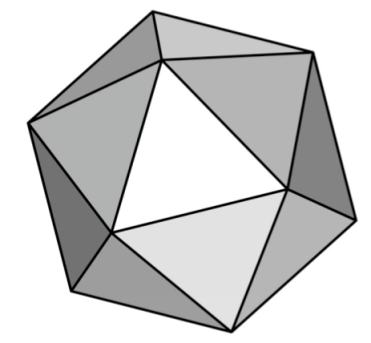
\includegraphics[width=0.7\textwidth]{icosahedron.png}
    \subcaption{}\label{fig_ico_a}
  \end{minipage}\hfill
  \begin{minipage}[b]{0.4\textwidth}
    \centering
    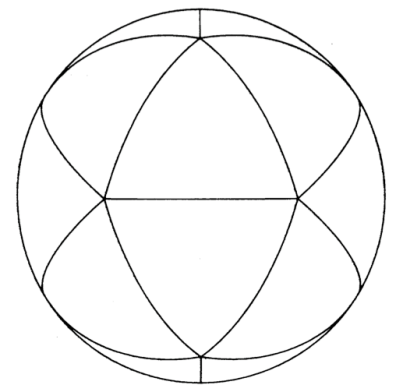
\includegraphics[width=0.7\textwidth]{icosahedron_spherical.png}
    \subcaption{}\label{fig_ico_b}
  \end{minipage}\hfill
  \caption{Icosahedron before (a) and after (b) projection onto a sphere }
\end{figure}

\begin{figure}[h]
  \begin{minipage}[b]{0.4\textwidth}
    \centering
    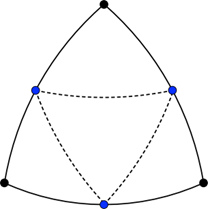
\includegraphics[width=0.7\textwidth]{bisection.png}
    \subcaption{}\label{fig_bisect}
  \end{minipage}\hfill
  \begin{minipage}[b]{0.4\textwidth}
    \centering
    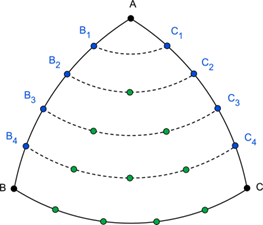
\includegraphics[width=0.8\textwidth]{nsection.png}
    \subcaption{}\label{fig_nsect}
  \end{minipage}\hfill
  \caption{(a) Bisection of the original triangle edges (b) More general division into $n$ equal sections}
\end{figure}

ICON grids are constructed by an initial root division into $n$ sections (\textbf{R}n) followed by $k$ bisection steps (\textbf{B}k), resulting in a \textbf{R}n\textbf{B}k grid. 
Figures \ref{fig_R2B00} and \ref{fig_R2B02} show \textbf{R}2\textbf{B}00 and \textbf{R}2\textbf{B}02 ICON grids. Such grids avoid polar singularities of latitude-longitude grids 
(Figure \ref{fig_lonlat}) and allow a high uniformity in resolution over the whole sphere.

\begin{figure}[h]
  \begin{minipage}[b]{0.3\textwidth}
    \centering
    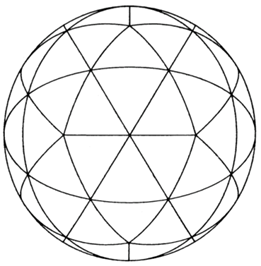
\includegraphics[width=0.9\textwidth]{icon_grid_R2B00.png}
    \subcaption{}\label{fig_R2B00}
  \end{minipage}\hfill
  \begin{minipage}[b]{0.3\textwidth}
    \centering
    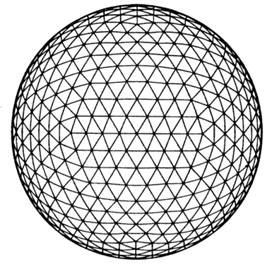
\includegraphics[width=0.95\textwidth]{icon_grid_R2B02.png}
    \subcaption{}\label{fig_R2B02}
  \end{minipage}\hfill
  \begin{minipage}[b]{0.3\textwidth}
    \centering
    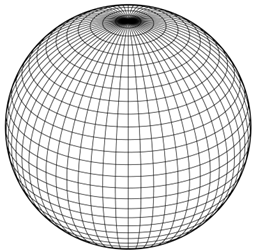
\includegraphics[width=0.95\textwidth]{lon-lat-grid.png}
    \subcaption{}\label{fig_lonlat}
  \end{minipage}\hfill
  \caption{(a) R2B00 grid. (b) R2B02 grid. (c) traditional latitude-longitude grids with polar singularities}
\end{figure}

Throughout this document, the grid is referred to as the ``\textbf{R}n\textbf{B}k grid'' or ``\textbf{R}n\textbf{B}k resolution''. For a given resolution \textbf{R}n\textbf{B}k, 
the total number of cells, edges, and vertices can be computed from
\begin{eqnarray*}
 n_{c} &=& 20\,n^{2}\,4^{k} \\
 n_{e} &=& 30\,n^{2}\,4^{k} \\
 n_{v} &=& 10\,n^{2}\,4^{k} + 2
\end{eqnarray*}
In Table \ref{tab_res}, some characteristics of frequently used ICON grids are given. The table contains information about the total number of triangles ($n_{c}$), the average 
distance between triangle cell centers (also referred to as the average resolution), and the maximum/minimum cell area. The latter may be interpreted as the area for which 
the prognosed meteorological quantities (like temperature, pressure, \dots) are representative.

\begin{table}[H]
  \caption{Characteristics of frequently used ICON grids. $\Delta A_{max}$ and $\Delta A_{min}$ refer to the maximum and minimum area of the grid cells, respectively.}\label{tab_res}
  \begin{center}
    \begin{tabular}{p{2.0cm}>{\raggedleft\arraybackslash}p{3.5cm}>{\centering\arraybackslash}p{3.5cm}>{\raggedleft\arraybackslash}p{2.5cm}>{\raggedleft\arraybackslash}p{2.5cm}}
    \toprule
    \textbf{Grid} & \textbf{number of cells ($n_{c}$)} & \textbf{avg.\ resolution [km]} & $\mathbf{\Delta A_{max}\,[km^{2}]}$ & $\mathbf{\Delta A_{min}\,[km^{2}]}$\\
    \midrule
    R2B04         &    20480                           &  157.8                         &  25974.2                  &  18777.3 \\
    R2B05         &    81920                           &   78.9                         &  6480.8                   & 4507.5\\
    R2B06         &   327680                           &   39.5                         &  1618.4                   & 1089.6 \\
    R2B07         &  1310720                           &   19.7                         &  404.4                    & 265.1 \\
    R3B07         &  2949120                           &   13.2                         &  179.7                    & 116.3 \\
    \bottomrule
    \end{tabular}
  \end{center}
\end{table}

\paragraph{}
\textbf{\textcolor{red}{The first operational version of ICON will most likely be based on the R3B07 grid, thus, having a horizontal resolution of about $13\,\mathrm{km}$!}}

\subsection{Local grid refinement}


\section{Vertical grid}